

\newglossaryentry{komponente}
{
    name=Komponente,
    description={Eine Komponente beschreibt in der Softwarearchitektur im Allgemeinen ein Teil eines Softwaresystems. Die Definition dieses Begriffs wird in speziellen Frameworks weiter spezifiziert. Bezogen auf das in der Arbeit verwendete EJB-Framework, werden bspw. die Beans als Komponenten betrachtet (vgl. \cite{ejbspec})}
}
\newglossaryentry{artefakt}
{
    name=Artefakt,
    description={Ein Artefakt beschreibt in der Software-Entwicklung die Spezifikation einer physischen Informationseinheit als Ergebnis des Software-Entwicklungsprozesses oder dem Deployment bzw. der Ausführung eines Systems. In der UML Spezifikation 2.1.2 \cite{uml} werden u.a. folgende konkrete Beispiele für Artefakte genannt:
    \begin{itemize}
    \item Dateien in denen Source Code enthalten ist
    \item Skripte
    \item Datenbanktabellen    
    \end{itemize}
    \noindent
    Im Kontext dieser Arbeit sind insbesondere die Dateien, in denen Source Code enthalten ist, allgemein als Artefakt bezeichnet}
}


\newglossaryentry{Engine}
{
    name=Engine,
    description={Eine Engine beschreibt eine Software oder einen Teil einer Software, der für eine spezifische Aufgabe verantwortlich ist (vgl. \cite{pcmag}). Die Aufgabe, die die in der Arbeit beschriebenen Source Engines erfüllen, wird in Abschnitt \ref{sec_tdcs} beschrieben}
}


\newglossaryentry{Interface}
{
    name=Interface,
    description={Ein Interface hat im Allgemeinen eine Übersetzungs- oder Vermittlungsfunktion zwischen gekoppelten Systemen (vgl. \cite{interfaces}). Die Bedeutung des Begriffs in dieser Arbeit bezieht sich jedoch auf den Kontext der objektorientierten Programmierung. In diesem Zusammenhang beschreibt ein Interface die Methoden, die in den Klassen, die dieses Interface erfüllen, vorhanden sein müssen}
}


\newglossaryentry{wrappertype}
{
    name=Wrapper-Typ,
    description={Ein Wrapper-Typ wird in der Programmierung auch als Hüllenklasse oder Adapter bezeichnet und entstammen dem \emph{Adapter-Muster} - einem Strukturmuster aus \cite{gof}. Eine solche Hüllenklasse beschreibt eine Klasse, mit der die Schnittstelle einer anderen Klasse angepasst werden kann. So ist es einem Klienten, welcher eine bestimmte Schnittstelle erwartet, möglich über die Hüllenklassen mit einer Klasse zusammenzuarbeiten, die die erwartete Schnittstelle nicht erfüllt. Die in dieser Arbeit beschriebenen Wrapper-Typen setzen dabei auf die Delegation der Schnittstellen-Anfragen. Das folgende Klassendiagramm zeigt die grundlegende Struktur solcher Wrapper-Typen. 
\begin{figure}[!h]
\centering
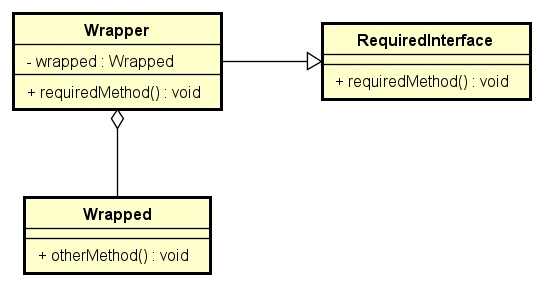
\includegraphics[width=0.75\textwidth]{cd_wrapper.png}
\label{bild}
\end{figure} 
    }
}

\newglossaryentry{JNDI}
{
    name=JNDI,
    description={Java Naming and Directory Interface (JNDI) ist eine API, welches den Entwickler*innen bei der Verwendung der Programmiersprache Java erlaubt, Referenzen von Objekten anhand eines Namens abzulegen und diese Objekte somit auch über den jeweiligen Namen zu adressieren. (vgl. \cite{jndi})}
}

\newglossaryentry{DependencyInjection}
{
    name=Dependency Injection,
    description={}
}

\newglossaryentry{injection}
{
    name=Injection,
    description={}
}

\newglossaryentry{attributgrammatik}
{
    name=Attributgrammatik,
    description={}
}

\newglossaryentry{substitutionsprinzip}
{
    name=Substitutionsprinzip,
    description={}
}

\newacronym{ast}{AST}{\Gls{abstractSyntaxtree}}


\newglossaryentry{abstractSyntaxtree}
{
    name=Abstrakter Syntaxbaum,
    description={}
}

\newglossaryentry{downcast}
{
    name=Downcast,
    description={}
}

\newglossaryentry{Heuristik}
{
    name=Heuristik,
    description={}
}

\newglossaryentry{bsort}
{
    name=Bubble-Sort,
    description={}
}

\newglossaryentry{Modul}
{
    name=Modul,
    description={}
}

\newglossaryentry{Komplexitaet}
{
    name=Komplexität,
    description={}
}


\newglossaryentry{Speicherkomplexitaet}
{
    name=Speicheromplexität,
    description={}
}


\newglossaryentry{Zeitkomplexitaet}
{
    name=Zeitkomplexität,
    description={}
}

\newglossaryentry{defaultmethode}
{
    name=Default-Methode,
    description={}
}
